During the second year of project activities integration activities
started. In the integration process, the architecture initially
presented in Deliverable D8.1 was deeply revised. This process was
required in order to align the activities carried out within the
project's technical work packages (WP2-WP7) and to ensure
interoperability among the components developed by the various
partners. In this section we briefly present the architecture as it
currently stands (at M24). No major changes are currently foreseen,
even if ---given the research-oriented nature of the SmartSociety
project--- this cannot be guaranteed. In this sense, the architectural
specifications of the SmartSociety platform have to be seen as a live document, which reflects the
actual progress of the research activities carried out by Consortium
partners. 

\subsection{Logical View}
A perspective view of the SmartSociety platform is reported in
Fig:~\ref{fig:perspective}. 

Two types of applications interact with the platform: User
Applications, which provide a service to (human) end users, and Peer
Applications, which are used to connect to peers (human or machine,
individuals or collectives) as a resource. 

User applications comprise both a client and server-side
component. The server-side component is considered part of the
platform. Applications need to be registered with the platform to
access its functionality. 

Peers (be them human or machines) need to be registered on the
platform to be able to provide resources, competences and services. 

External sources and external services may interact via the
SmartSociety platform via appropriate connectors. 

\begin{figure}
\centering
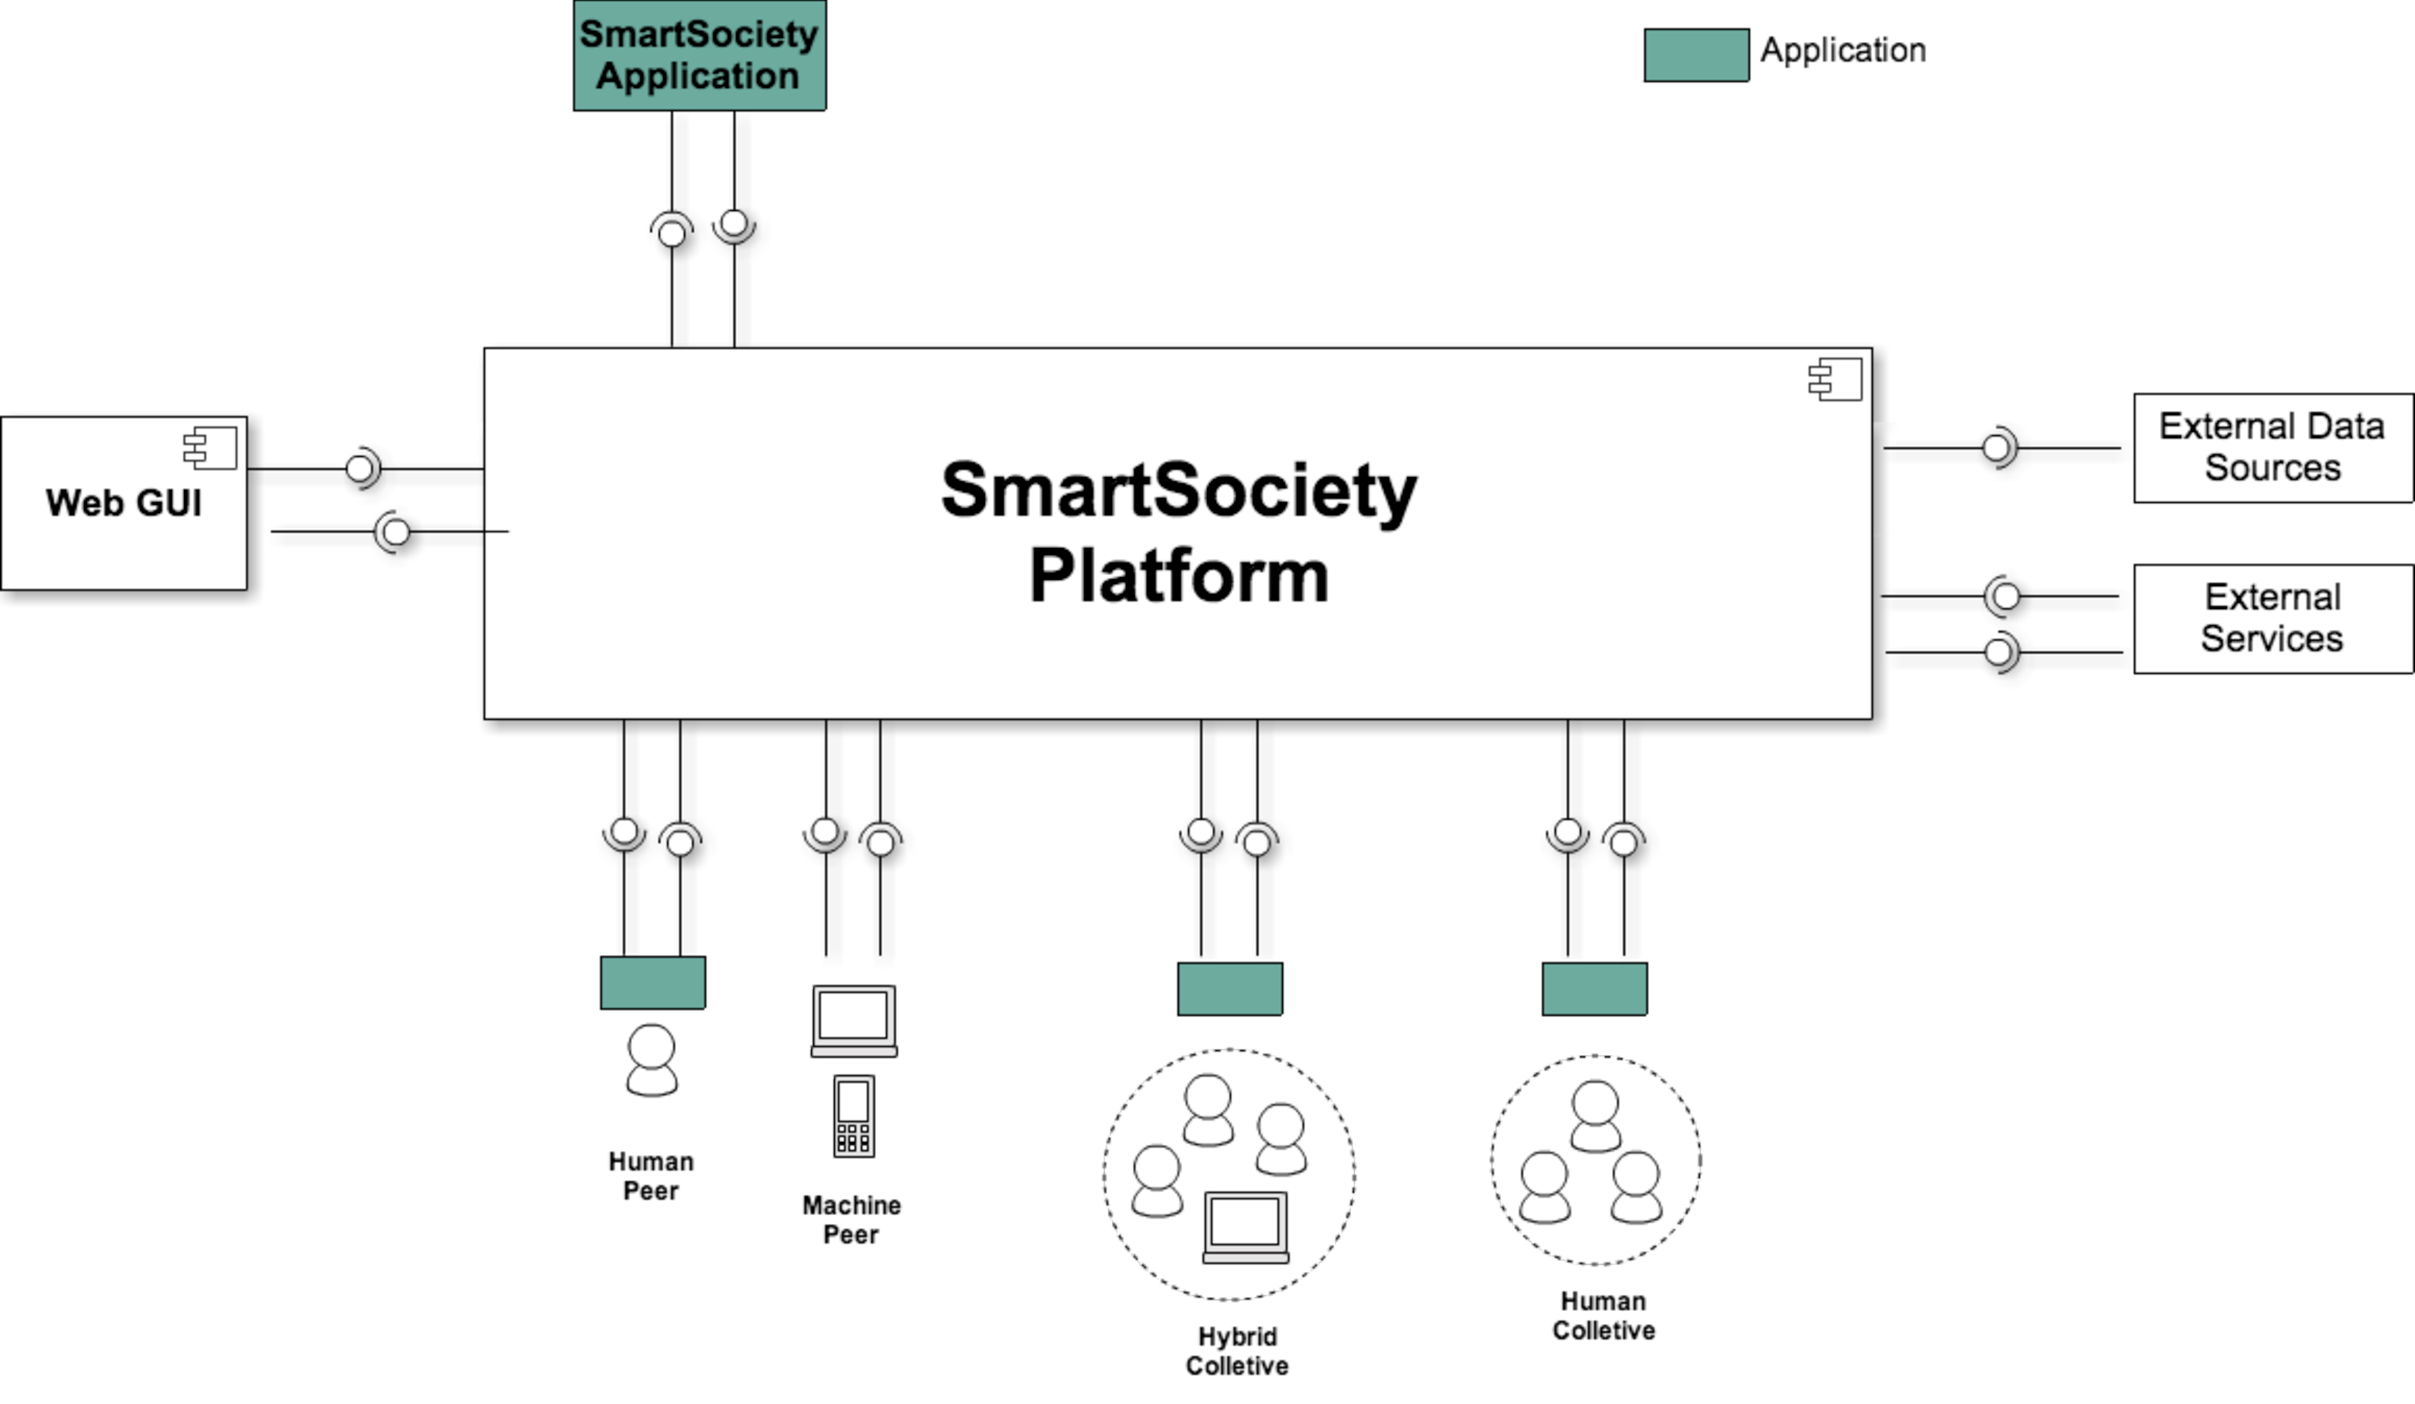
\includegraphics[width=0.9\textwidth]{./figs/perspective_view}
\caption{Perspective view of the SmartSociety platform.}
\label{fig:perspective}
\end{figure}

A functional diagram of the SmartSociety platform is reported in
Fig:~\ref{fig:functional}. The Consortium has identified 9 key
components which jointly provide the required functionality:
\begin{itemize}
\item Knowledge base:it contains an agreed ontology about peers, task,
workflows, incentives, etc. and it is used for ensuring semantic
interoperability among the other platform components. 
\item Provenance store: it logs actions performed by platform
components and peers according to the W3C PROV recommendation. It
further supports an auditing service which is able to reconstruct and
visualize provenance trails. 
\item Peer manager:it is in charge of managing the peers that are part
of the SmartSociety system. It maintains a profile of each peer, which
represents a model thereof in terms of knowledge, resources and
capacity. It provides a peer search functionality that allows other
components to find for the most appropriate peers for a given tasks. 
\item Context manager: it dynamically monitors the context the human
peers are in (in terms of, e.g., location, activity etc.). This
information is fed to the peer manager and represents the dynamic part
of the peer profile. 
\item Incentives manager: it provides insight on incentives and
interventions that can be used to achieve higher quality results. 
\item Orchestration and coordination manager: it provides two key
functionalities: composition and negotiaton. Composition takes as
inputs tasks and interacts with the peer manager to find suitable
peers for completing the task. The negotiation manager is in charge of
handling the negotiation process with peers in order to ensure that
the necessary services and resources required to carry out the task
can be guaranteed. 
\item Reputation manager: it computes the
reputation of a given peer based on feedback from users. It uses data
from the provenance store in order to carry out the computation.
\item Monitoring and analytics service: this service logs and monitors
the platform jobs and can be used by platform administrators to
perform root-cause analysis and to extract analytics on the
performance of the system. 
\item Elasticity manager:
\item Communication middleware: 
\end{itemize}       
\begin{figure}
\centering
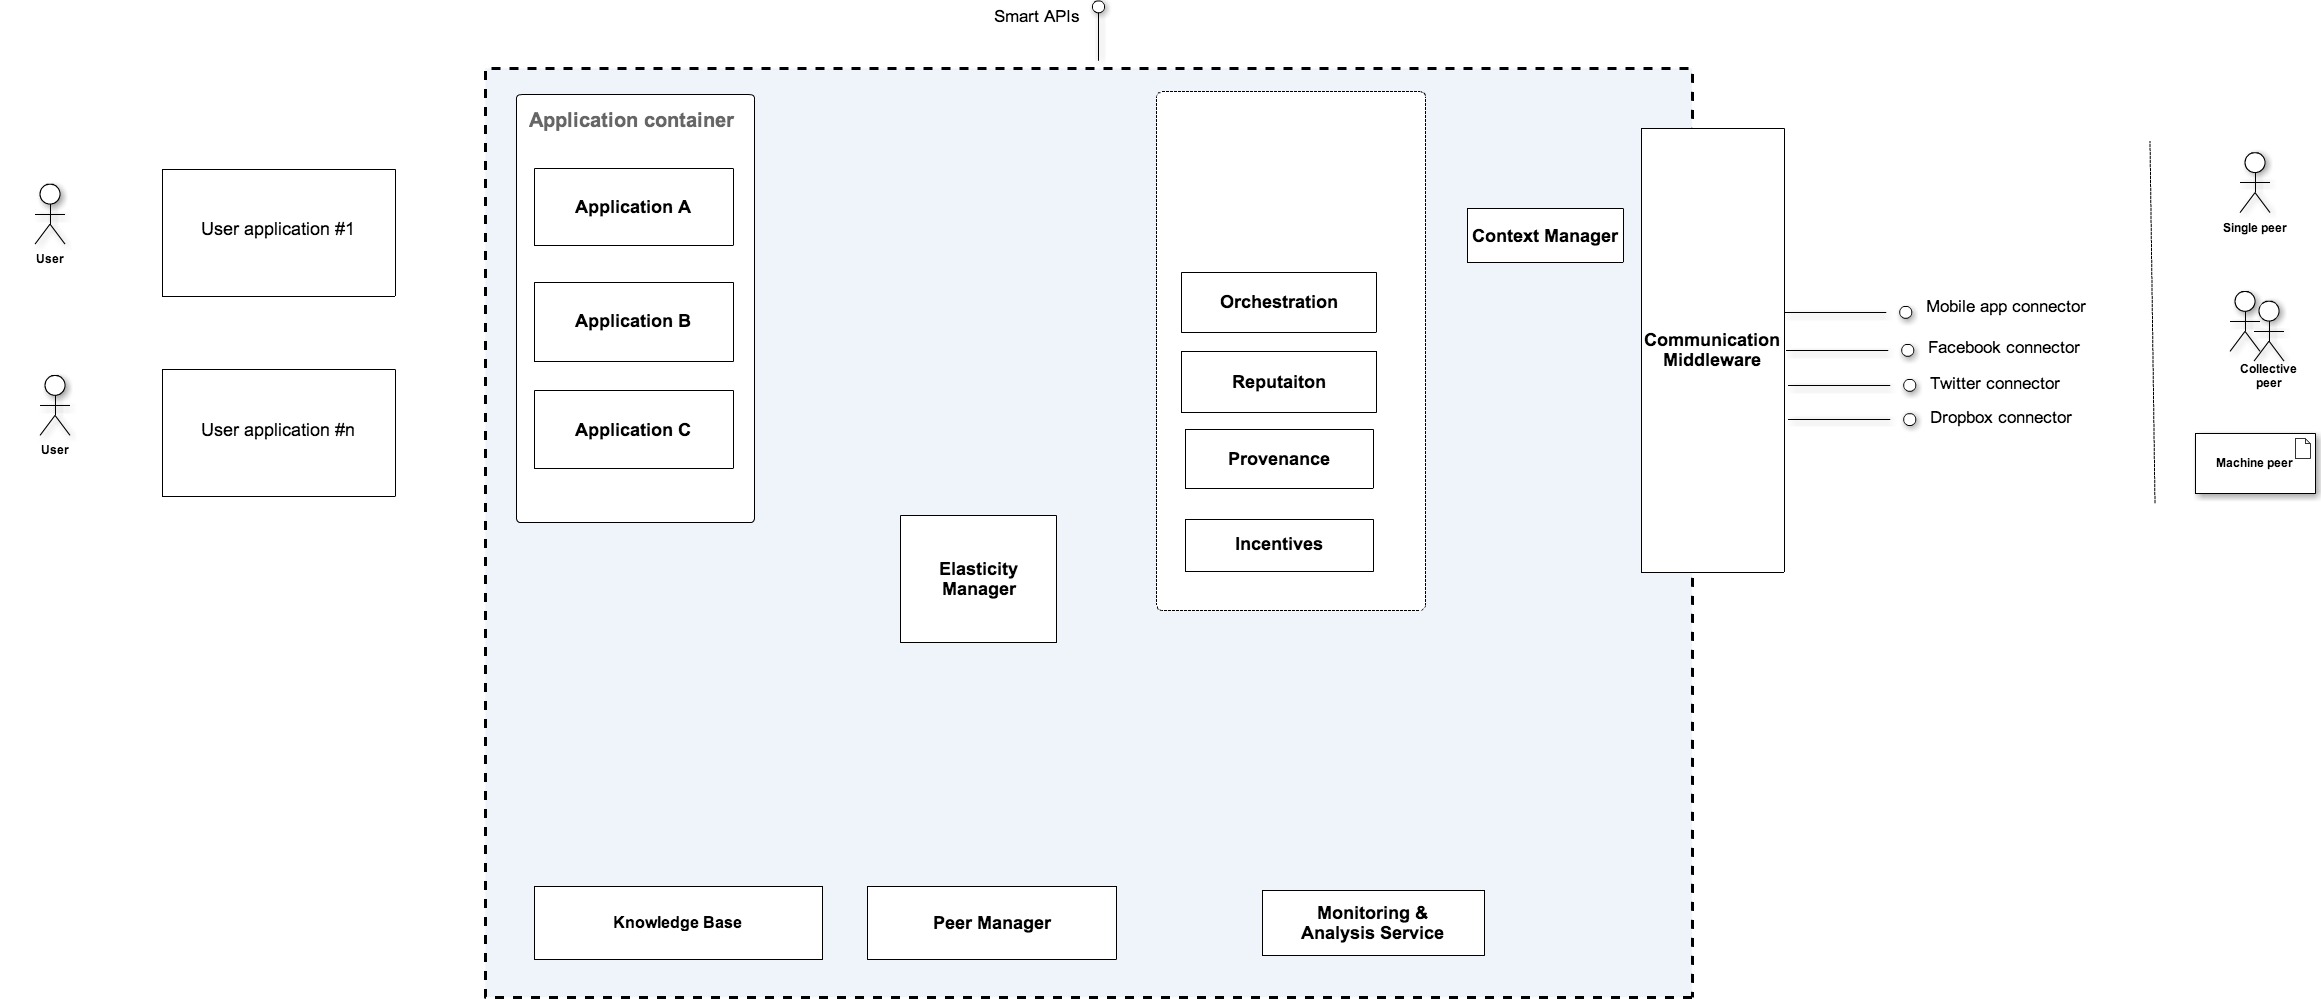
\includegraphics[width=0.9\textwidth]{./figs/functional_diagram}
\caption{Functional diagram of the SmartSociety platform
architecture.}
\label{fig:functional}
\end{figure}

\subsection{Deployment View and Network Diagrams}
The SmartSociety platform has been designed around a REST architecture
with the aim of supporting flexibility in the deployment model. This
means that the platform shall seamlessly support both single-tenant as
well as multi-tenant deployment models. Also, the platform component
can be centralised on a single infrastructure or can be distributed
across different servers. The choice of the specific deployment model
to be used depends on technical as well as business considerations. In
the remainder of this section we present, as a use case, the current
deployment utilised for integration, testing, validation and
experimentation purposes. This is by no means to be considered the
only model supported, but it provides an actual example of the
supported configuration. 

\subsection{Dynamic View}
The SmartSociety platform is meant to support a rather wide range of
social computation patterns (or templates). In order to provide
insight into the flexibility of the platform and the actual
interworking of components, we have developed sequence diagrams for two
'extreme' applications:
\begin{itemize}
\item SmartShare is a ridesharing system able to account for user's
preferences and to compute recommendations based on the feedback
provided by other service users. It is what we call a 'full
negotiation' scenario, in which the computational task of finding an
agreement on the rides is left to individuals and collectives. The
platform in this case is used to carry out administration tasks, in
particular keeping track of the rides and ride requests, their status
and to maintain reputation of drivers and passengers.
\item AskSmartSociety! is a Q\&A service supporting hybridity. The
computational pattern here is that typical of micro-tasking
applications (\'a la Mechanical Turk, roughly speaking), where the
task in this corresponds to a question to be answered. The service
supports hybrid computation in that questions can be transparently
provided by machine peers or human peers. Quality criteria can be
specified in order to define when a chosen answer has to be presented
to the user. 
\end{itemize}
In the following we present details about the two aforementioned
applications. 
\subsubsection{Example: SmartShare}
\begin{figure}
\centering
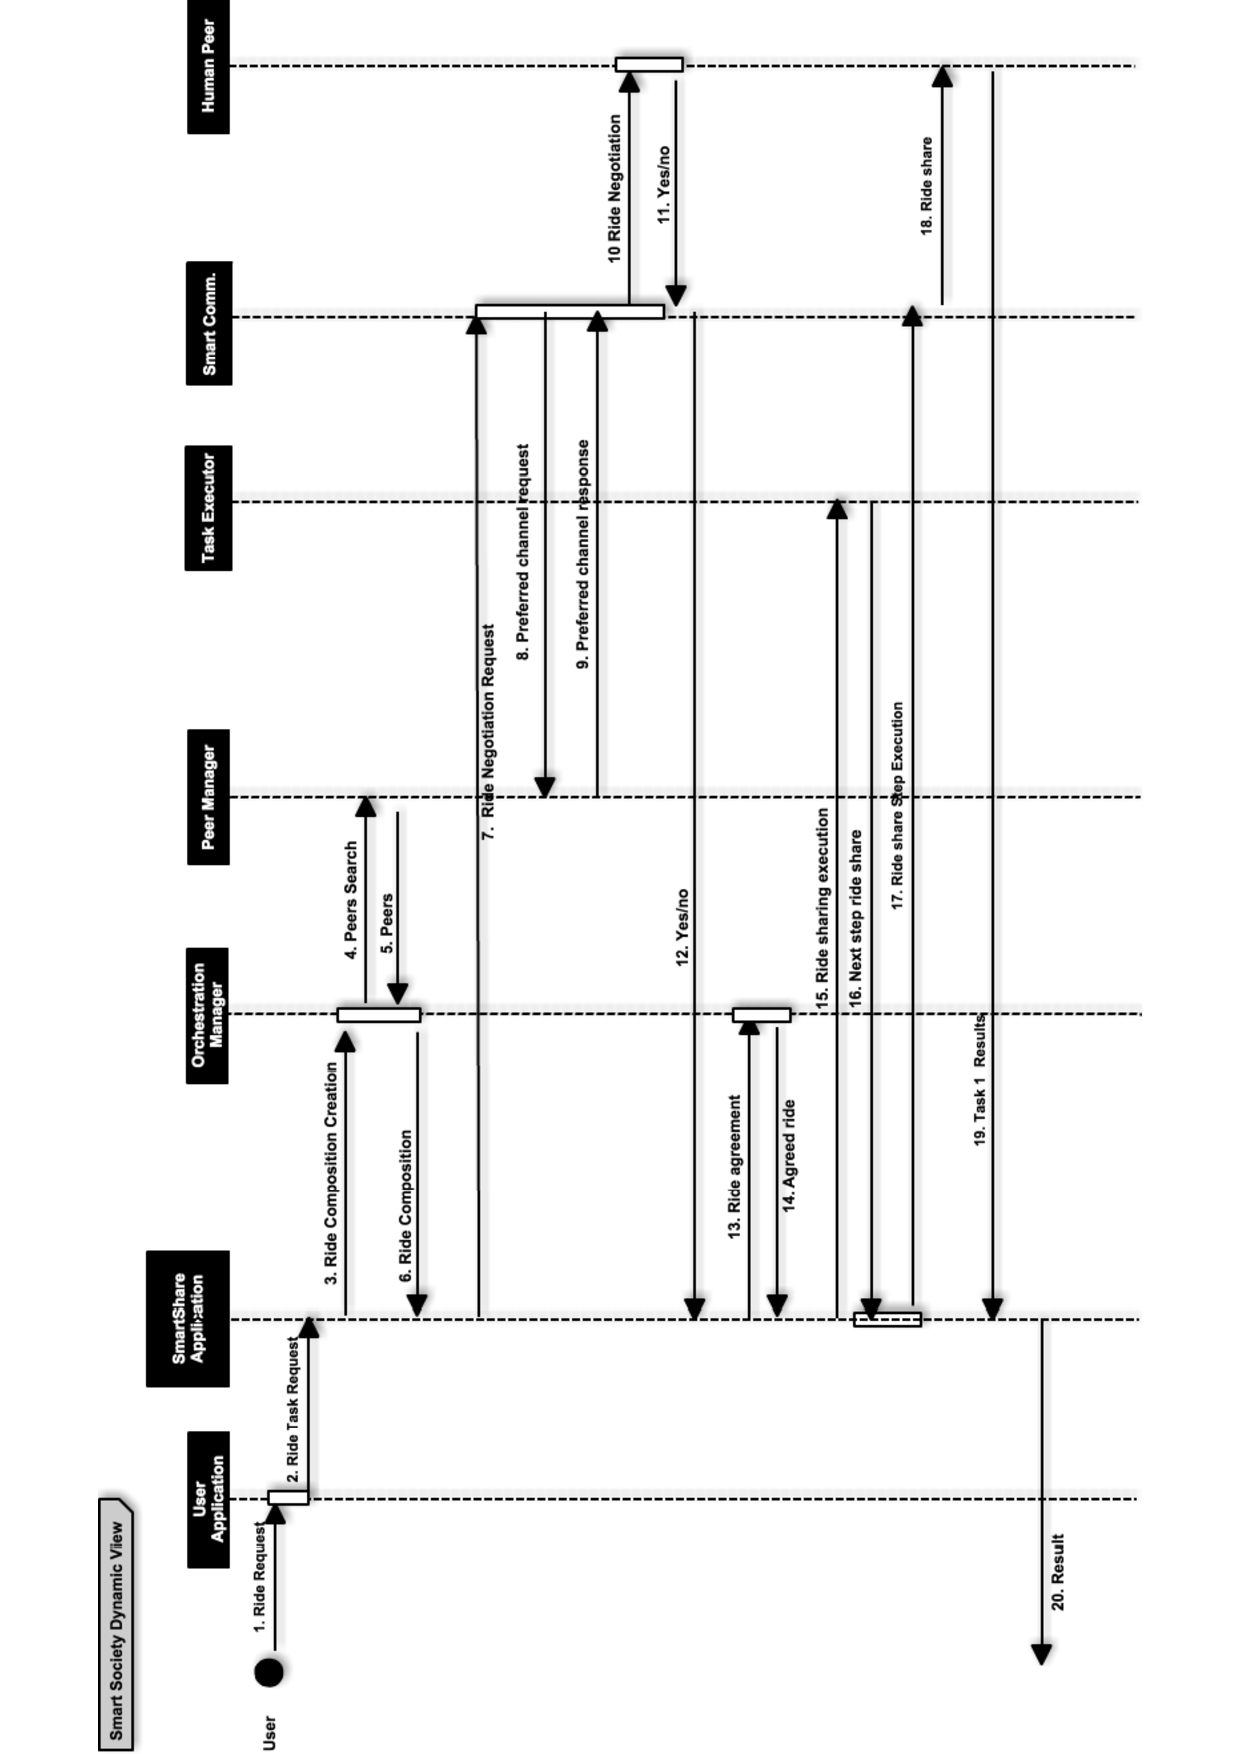
\includegraphics[width=0.9\textwidth]{./figs/sequenceRide}
\caption{Sequence diagram of the SmartShare application.}
\label{fig:dynamic_share}
\end{figure}
\subsubsection{Example: Ask SmartSociety!}
\begin{figure}
\centering
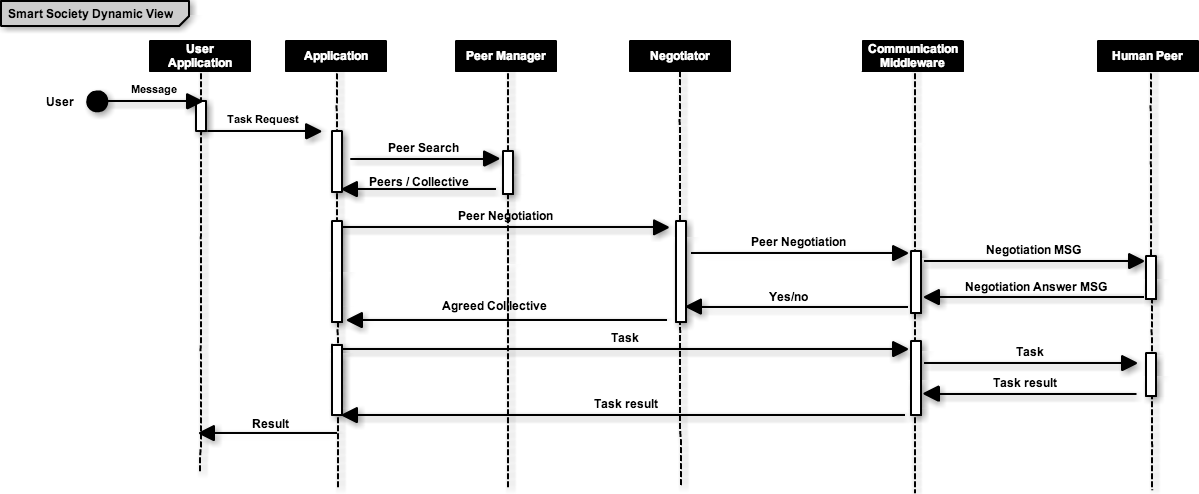
\includegraphics[width=0.9\textwidth]{./figs/sequenceAsk}
\caption{Sequence diagram for AskSmartSociety! applications.}
\label{fig:dynamic_ask}
\end{figure}